\chapter{Modeling Results}\label{ch:results}
Until now we have only looked at the behavioral data. We have found that time pressure reduces the reaction time, has an effect on which arm is chosen (e.g. the least risky one) and reduces the choice diversity. The behavior suggests that time pressure indeed has an influence on the uncertainty bonus in bandit problems, which results in the reported behavior. \\
In order to gain a better understanding of the guiding process, we will turn to modeling the participants' behavior. By modeling human behavior, we can have a better look how time pressure influences the uncertainty bonus of directed exploration. We hope to see a difference in the exploration parameter $\beta$ in the UCB for unlimited and limited time rounds. 
%Remind the reader what's happening here. We've reported  behavioral results but now we want to turn to modeling to get a better understanding of behavior. What are the main questions? (e.g., how does time pressure influence the uncertainty bonus)

\section{Modeling Results}
In the following sections we will focus on the different models we have used and their predictive accuracy (e.g. how well they predicted the participants' choices). Then we will take a look at the different parameter estimates, which will give us more insight in the understanding of the behavior. Finally, we will simulate the participants data with the models in order to see if a similar learning curves as in our participant data can be recreated. 
%Explain to the reader first the order of this chapter. We compare different models in their out-of-sample predictive accuracy. Then we look at parameters to understand their behavior. And then we simulate learning curves as a posterior check on the validity of our models

\subsection{Model Comparison}
%Explain how we compared the models (cross validation, out of sample log loss, reported as McFadden pseudo-R2, report t-tests, number participants best explained)
We used two different learning models, the Kalman filter and an simpler version of it: the BMT. The two learning models differ in the way that the KF not only tracks the mean but also the variance, while the BMT works with the assumption of a know variance. The innovation variance which the Kalman filter has, but the BMT lacks, is a measure of how much uncertainty grows for options that were not chosen. The error variance, that both models have, shows an inverse sensitivity to the observed rewards, e.g. it determines how large the update for the next trial will be. 

These two learning models were paired with four sampling strategies: the UCB, the linear model, the Thompson sampling and the hybrid model.
The UCB is a representative of directed exploration, e.g. it works with an uncertainty bonus and thus "directs" the agent to more uncertain options to gain more knowledge. This uncertainty bonus or exploration bonus is represented in the parameter $\beta$ or $\beta_{sig}$
The linear model, which is a variation on the UCB does not contain a bonus on the variance but also on the mean which is then called $\beta_{mu}$.

The Thompson sampling lies between random and directed exploration; while it prefers the option with the best outcome, randomness is still added in order to create some exploration. 

The Hybrid model is a combination of the Thompson sampling and the UCB, it considers the exploration parameter $\beta$ while sampling and computing the choice probability the same way as the Thompson sampling. 

%Summarize the parameters that are fit and what they mean
%Then also introduce the stickiness parameter here and justify it based on your behavioral analysis of choice repeats
We implemented an additional parameter in each of the four exploration strategies\citep{gershman2009human}. The "stickiness" parameter $\omega$ is a weight on the previous choice for the calculation of the new probabilities (and thus for the next choice).

%Report Cross validated maximum likelihood estimates
We calculated the parameters with a leave one out cross validation method and in it an optimization algorithm based on differential evolution\citep{DEoptim}. 
Cross validation is a method that uses a training and a test set in order to calculate a loss.
During the first phase, the parameters are fitted onto the training set, which consists of 19 rounds of the same time condition. 
The test set or validation set, which consists of the remaining one round of that time condition, is then used to see how well the fitted model does in terms of prediction. We use the estimated parameters of the 19 rounds on the one test round, from which we calculate the log likelihood with the help of a loss function. 
%Explain psuedo-R^2
The $R^2$ is a goodness of fit measure and gives us information of how well the model predicted the data. It usually ranges in an interval between zero and one. It can occur that some models have values below zero, which is the case when the the model performs worse than just randomly picking an option (in our case). When the $R^2$ value is equal to one, the model predicts the data perfectly. We calculate it by summarizing the log likelihood of each round per participant and divide it by the random model, which gives a probability of $0.25$ to each option.
Figure ~\ref{fig:R2ConditionsPayoff} shows the $R^2$ values of each model separated by time condition. 
\begin{figure}
    \centering
    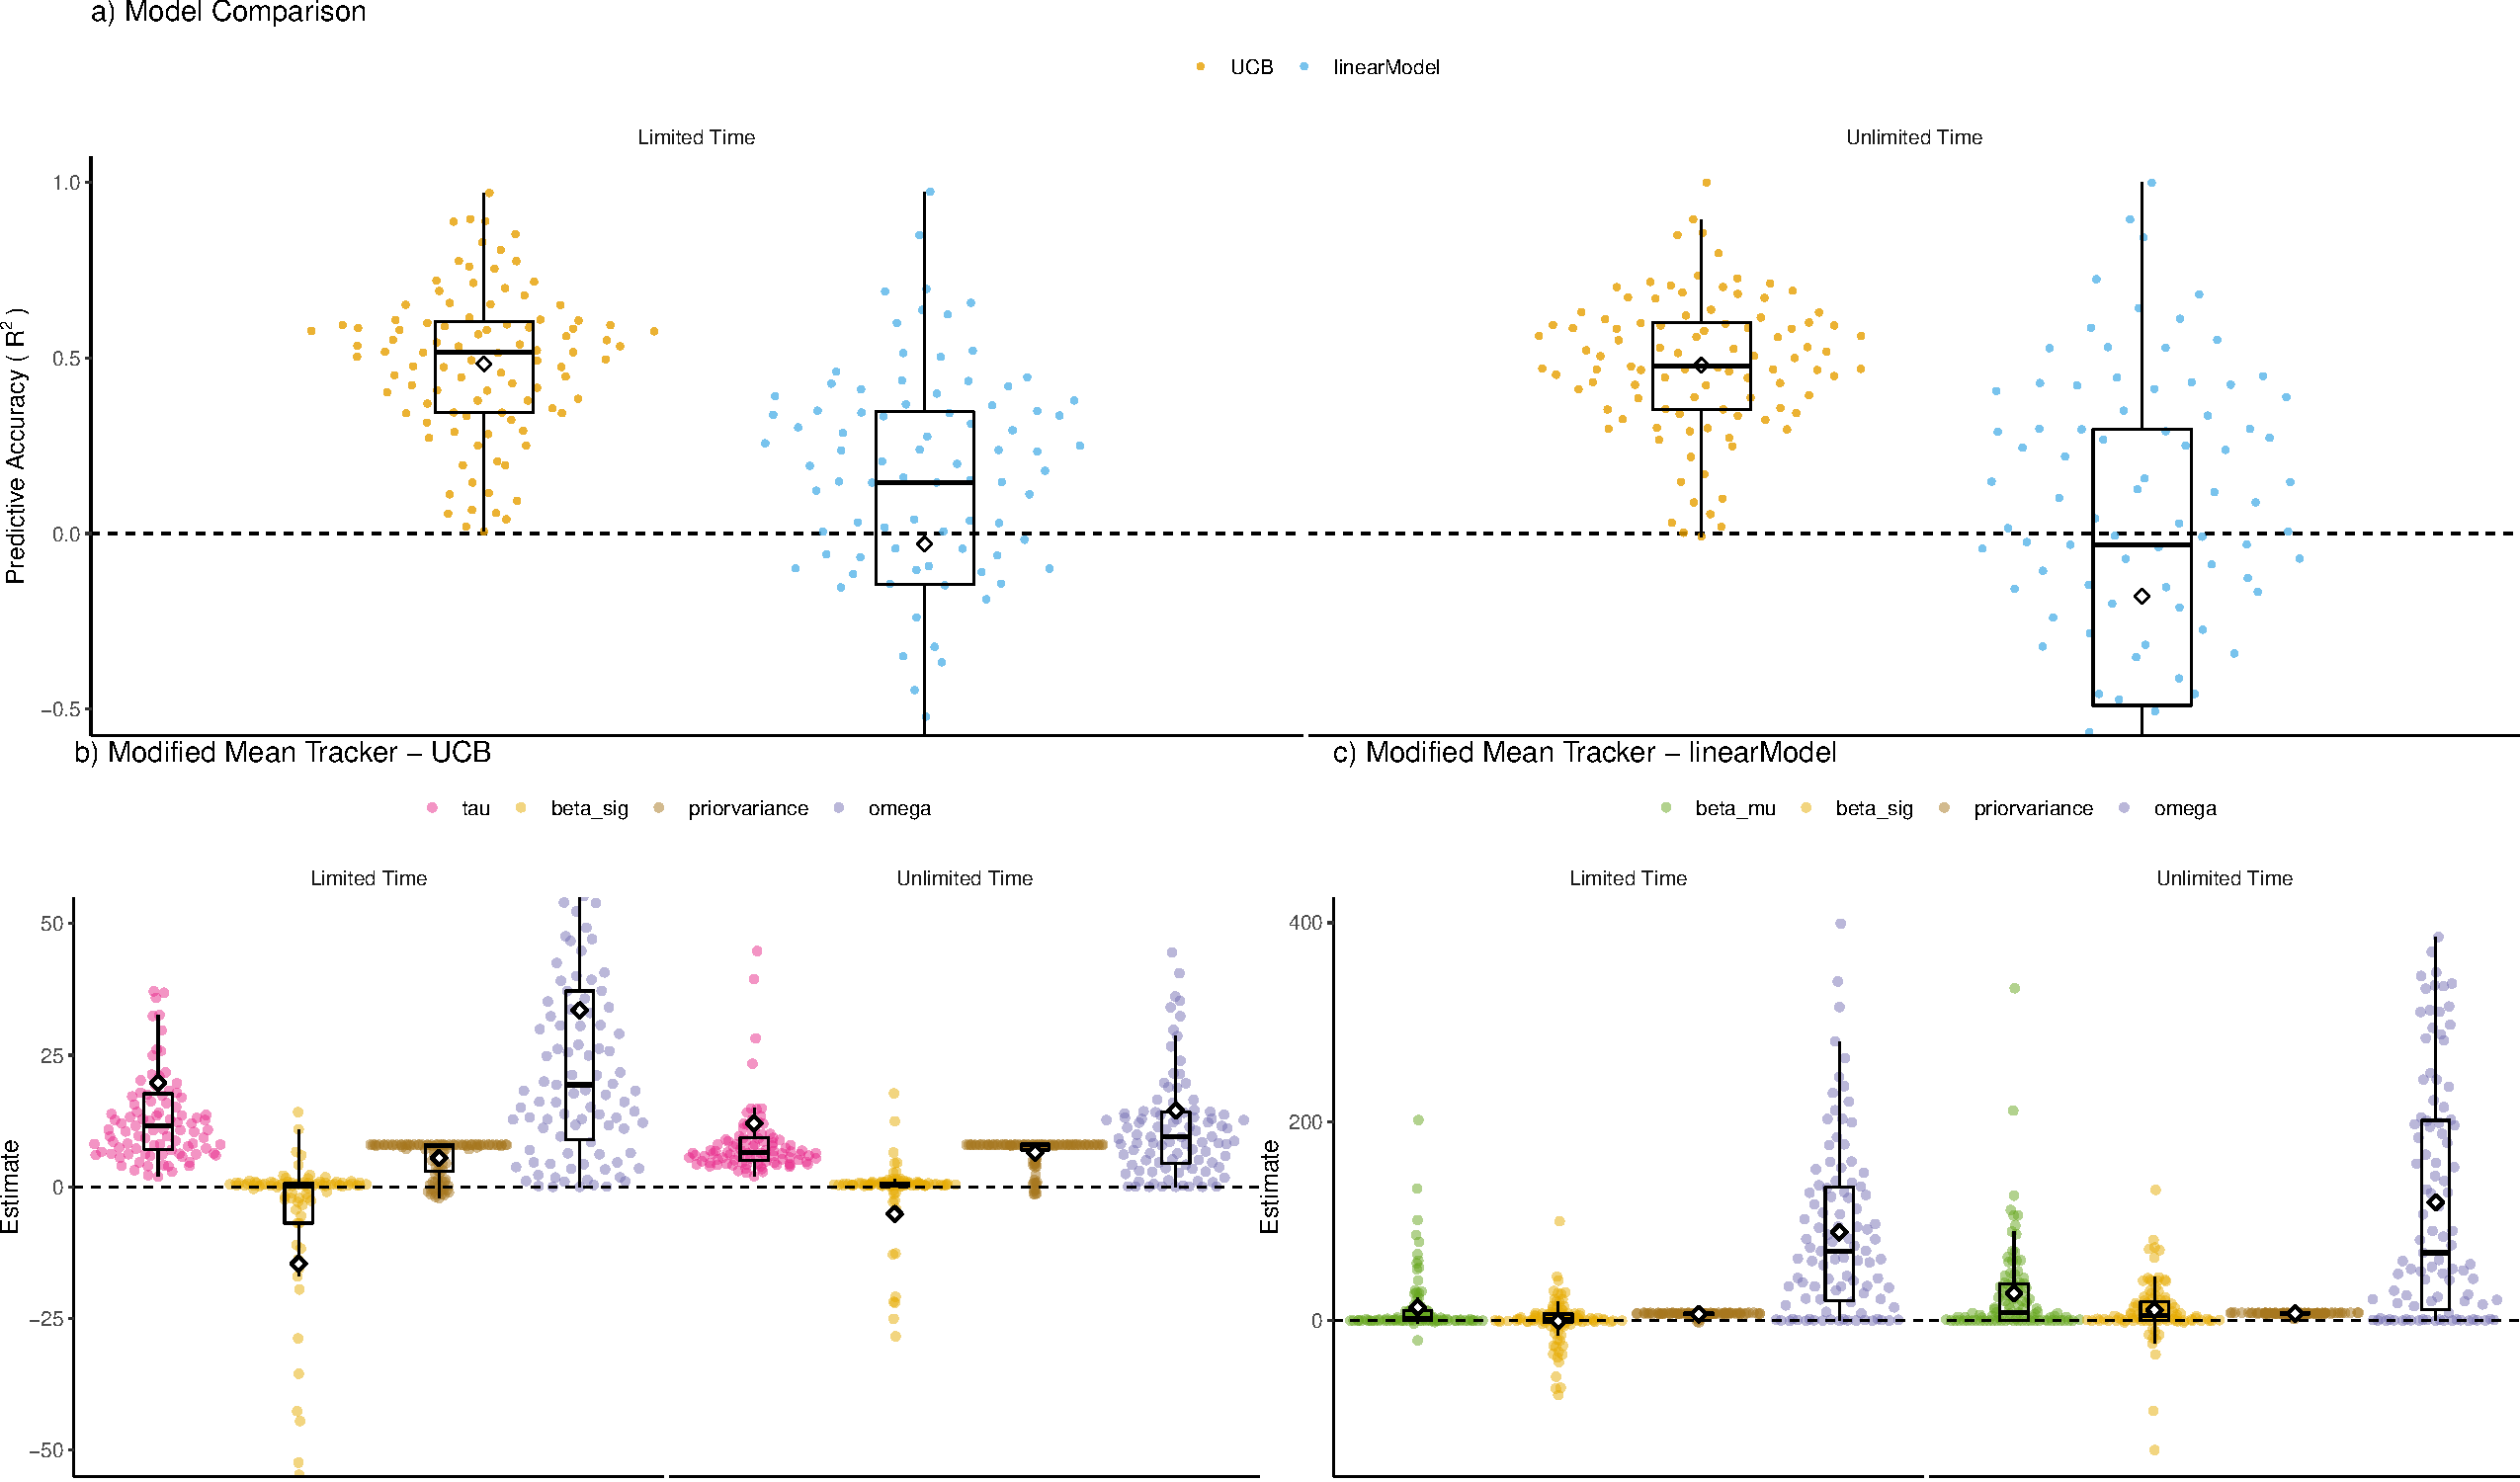
\includegraphics[width=1\textwidth]{Plots/ModellingResults.pdf}
    \caption[Modeling Results for the Modified Mean Tracker]{a) }
    \label{fig:R2ConditionsPayoff}
\end{figure}
%Model Comparision 
There was a significant difference in the $R^2$ values for the two sampling strategies. The UCB performed better than the linear model ($t(197)=-13.7, p<.001,d=0.97, BF>100$).  
%Model + UCB vs Model +UCB -- model comaprison 
%There was no significant difference in the $R^2$ values for the two learning models when using the UCB strategy ($t(98=1.057$, $p=.293$, $d=0.106$, $BF=0.19$), the same holds for the Thompson sampling ($t(98=-2.9$,$p=.004$, $d=0.3$, $BF=6.62$).
% Sampling Strategy comparison
%However, UCB performs better than Thompson sampling for both the KF ($t(98)=8.09, p<.001, d=0.81, BF>100$) and the BMT ($t(98)=5.5,p<.001, d=0.55, BF>100$). 
%The Hybrid model performs worse than the UCB with the BMT model ($t(98)=5.7, p<.001, d=0.57, BF>100$).
%report here for Kalman filter and Hybrid model vs UCb
%There was no significant difference in performance for between the Hybrid model and the Thompson sampling (KF:, BMT: $t(98)=2.1, p=.04, d=0.21, BF=0.9$).

\subsection{Parameter estimates}
\paragraph{Stickiness parameter}
We included another parameter, the so called stickiness parameter $\omega$. It is a parameter that weights the last chosen option. 
%Focus on best model, report median parameters, do non-parametric tests (paired!), analyze what the differences mean (e.g., uncertainty bonus, etc...)%Focus on best model, report median parameters, do non-parametric tests (paired!), analyze what the differences mean (e.g., uncertainty bonus, etc...)
\paragraph{Cross validation results with Stickiness parameter}
The modified BMT combined with the UCB was the best fitting model for 92 participants, where 7 also had the best fit for the Modified BMT linear model combination.
%The KF-UCB combination proved to be the best fit for 40 participants. For a complete overview see Appendix B ~\ref{tab:All_Fitted}. 
In the following we will report the median parameters for the overall best model (see Table ~\ref{tab:BMTUCBparams}). The best model fit did not change over the different Time Conditions.
\begin{table}
    \vspace{-2mm}
    \begin{tabular*}{\textwidth}{@{}l@{\extracolsep{\fill}}cccc@{}}
         Time Conditions & $\beta$ &$\tau$ &$\omega$ & priorvariance  \\ \midrule
         All & $0.35$  & $8.1$&$12.97$ & $8$\\
         Unlimited Time & $0.42$ & $6.42$ & $9.64$ & $8$  \\
         Limited Time & $0.28$ & $11.33$ & $20.88$ & $8$ \\
         \bottomrule
    \end{tabular*}
    \vspace{5mm}
    \caption{Median Parameters for modified BMT - UCB combination for best fitted models}
    \label{tab:MedianMBMTUCBbest}
\end{table}
%here over all participants MEan and median over all Participants
\begin{table}
    \vspace{-2mm}
    \begin{tabular*}{\textwidth}{@{}l@{\extracolsep{\fill}}cccc@{}}
         Time Conditions & $\beta$ &$\tau$ &$\omega$ & priorvariance  \\ \midrule
         All & $-9.7|0.35$  & $15.6|8.2$&$23.97|12.87$ & $5.66|8$\\
         Unlimited Time & $-4.81|0.422$ &$11.91|6.65$ & $14.75|9.25$ & $6.33|8$  \\
         Limited Time & $-14.58|0.28$ & $19.26|11.05$ & $33.18|18.5$ & $4.98|8$ \\
         \bottomrule
    \end{tabular*}
    \vspace{5mm}
    \caption{Median Parameters for modified BMT - UCB combination over all participants}
    \label{tab:MedianMBMTUCBALL}
\end{table}
%\begin{table}
%\vspace{-2mm}
%\caption{Median Parameters for BMT - UCB combination overall participants} 
%\label{tab:BMTUCBparams} 
%\begin{tabular*}{\textwidth}{@{}l@{\extracolsep{\fill}}cccc@{}}
%\toprule
%Time Conditions & $\beta$ &$\tau$ &$\omega$ & $\theta_\epsilon^2$  \\ \midrule
%All & $0.017$  & $10.57$&$27.3$ & $14.56$     \\
%Unlimited Time   & $0.0171$ & $10.57$ &$22.4$& $15.5$      \\
%Limited Time & $0.0169$ & $10.56$ &$33.3$&    $13.62$   \\
%\bottomrule
%\end{tabular*}
%\vspace{5mm}
%\end{table}
%non parametric test
We applied non-parametric test on the different parameters for Unlimited versus Limited Time conditions. We used the Wilcox-signed ranking test, because we assume that the parameters are not normally distributed. The test evaluates if the ranks of the two means differ, e.g. if the parameters come from the same distribution. 
If we consider the parameters for the modified BMT with the UCB we found that $\beta$ differed significantly between unlimited and limited time rounds ($Z=-3.5$, $p<.001$, $r=-.35$, $BF>100$). The priorvariance did not differ significantly ($Z=-1.9$, $p=.028$, $r=-.19$, $BF=4.1$).
%For each parameter of the BMT-UCB combination, we did not find any significant difference between Unlimited and Limited Time ($\beta$: $Z=-1.4$, $p=.086$, $r=-.07$, $BF=.40$, $\tau$: $Z=1.0$, $p=.846$, $r=.05$, $BF=.06$, $\omega$: $Z=-0.5$, $p=.311$, $r=-.02$, $BF=.10$,$\theta_\epsilon^2$:$Z=1.2$, $p=.891$, $r=.06$, $BF=.06$).

%analysing the different parameters
%median parameters
The median for exploration factor $\beta$ was $0.017$, for Unlimited and Limited Time see ~\ref{tab:BMTUCBparams}. However, for the best fitted models the median exploration factor was at $3.04$, furthermore in the best fitted models the beta value for Limited Time Conditions was $2.2$, while for Unlimited Time it was at $8$ (for a complete overview of the parameters for the best fitted models see Appendix B ~\ref{tab:AllbestParam}). This shows, that for the best fitted models, we can see a difference in the exploration for the different Time Conditions, e.g the models suggest that participants explore less in Limited Time Conditions. Interestingly, this is not the case for the IGT condition in which the best fitted models have a higher $\beta$ for the Limited Time Condition.

The error variance  $\theta_\epsilon^2$, describes the sensitivity towards the observed rewards, e.g. it weights the observed data. Remember, if it is low then it will make larger updates for the next prediction. Considering only the best fitted models, we can see a difference between Unlimited and Limited Time, where  $\theta_\epsilon^2$ is smaller during Unlimited Time Conditions (overall as well as in each Payoff Condition), which suggests that the model is less sensitive to new information. 
Intuitively speaking, if you have less time to explore or compute, then it makes sense to give more weight to new information in order to be faster to decide for the next trial.

The temperature parameter $\tau$ shows how similar the probabilities of the different options are. Again, if we consider only the best fitting models, then we see that $\tau$ is higher for Unlimited Time Rounds with a median of $43.7$, while Limited Time Rounds have a median of $21.2$. The higher values indicate a that the probabilities of the different options are very similar. 

Lastly, the stickiness parameter $\omega$, which we included as a weight for the last choice. For most conditions, we see that the stickiness parameter is higher for unlimited rounds than for limited rounds. This indicates that during unlimited time rounds the very last choice has more weight than during limited time rounds. This does not necessarily contradict $\theta_\epsilon^2$, since $\theta_\epsilon^2$ speaks over the overall update, it is however possible that the last choice gives more weight in this update. 


\subsection{Learning curves}
In order to see how well our models and parameters perform, we implemented a simulation of the experiment with the models as participants. 
To gain a similar data set, we created an environment that was able to simulate the participants data. To create the same amount of data, we extracted the parameters for each participant for each time condition condition for only the best fitting model. 
In order to gain 20 rounds of 20 trials each, we first looped through 5 rounds before taking the parameters of the next condition combination and loop through this 5 times again. Within the 5 rounds, we looped through the 20 trials, on the first trial, we randomly assigned one option to sample from. 
A rewards was sampled according to the experiment, with the same number that manipulated one of the according rounds added to the rewards. The model updated based on this new reward and then in order to produce a new choice. 
%we looped through the number of participants, though each Time and Payoff Condition and extracted the parameters of either 1) the best fitting model for the combination for the BMT-UCB or 2) for each participants best fitted model (either BMT-UCB or KF-UCB) for that combination. For the first decision we randomly sampled a decision between 1 and 4 to get the first chosen option and a reward. Based upon this we let our learning model learn the outcome and updated it. For the second and each following trial, we calculated the posterior with the model, which is then used to calculate the probabilities for the decision with the exploration strategy. From this probability distribution over the options, we took the highest one as the chosen option. With this option we were able to sample the rewards according to the experiment. This updated again for 20 trials. 
We gained 
%Describe the simulation procedure, describe the qualitative results

\subsection{Recoverability}
In order to verify our parameters, we recovered them by simulating the participants behavior with the estimated parameters and the models. This created a dataframe similar to the participants behavior, which we use to run our crossvaldiaton over it in order to gain similar parameters. 

%We take out models, simulate behavior, and then run our modeling procedure on the simulated data. 1. Model recovery. Do we recover the correct generating model based on the simulated data? this tells us that our model comparison method can properly distinguish the different models. 2. Parameter recovery. Do we recover correlated parameters? This shows that the parameters we estimate are meaningful and separate, rather than arbitrary

